\chapter{Background}\label{sec:bknd}

Here we will briefly describe some background concepts and ideas that will aid and facilitate discussion of subset identification in later chapters.

\section{General Notations}
The following notations will be standard and followed consistently throughout the sequel, unless otherwise noted.
\begin{itemize}
\item Calligraphic capital letters will typically represent spaces, and capital letters will typically represent an instance or element from those spaces.

\item Set sizes will typically take the form of lowercase $n,d,p$, generally associated with the number of samples, the dimension of some feature space, and the number of parameters respectively. $i,j,k$ will be used for indexing various sets within context.

\item We use $\RR^d$ to represent $d$-dimensional vector space over the reals, and vectors will be lowercase typically as $x,y,z$ and matrices and higher order tensors will be denoted in uppercase, with local clarity on their distinction between a set instance.

\item $S$ will denote a of training examples.
A sample $s_i\in S$ may be indexed by $i \in [1,\ldots,n]$. 
For general and generative settings, $x_i$ may be used in place, and for predictive settings will be represented by the tuple $s_i:=(x_i,y_i)$.

\end{itemize}

\section{Differential Geometry}
Here we present a brief overview of differential geometry. For a more in depth background, we refer interested readers to \cite{do1992riemannian},\cite{lee2003smooth}, and \cite{spivak1981comprehensive}.


%Before discussion about general regressions models for manifold-valued response variables, let's revisit manifolds.
\textbf{Differentiable manifold.}
A \textit{differentiable (smooth) manifold} of dimension $n$ is a set $\Mc$ and a maximal family of \textit{injective} mappings $\varphi_{i}:U_{i}
\subset \textbf{R}^{n} \rightarrow \Mc$ of open sets $U_{i}$ of
$\RR^{n}$ into $\Mc$ such that:
\begin{enumerate}
\item $\cup_{i}\varphi_{i}(U_{i}) =\Mc$
\item for any pair $i,j$ with $\varphi_{i} (U_{i}) \cap
\varphi_{j} (U_{j}) = W \neq \phi$, the sets $\varphi_{i}^{-1}(W)$
and $\varphi_{j}^{-1}(W)$ are open sets in $\RR^{n}$ and the
mappings $\varphi_{j}^{-1} \circ \varphi_{i}$ are
differentiable, where $\circ$ denotes function composition. 
\item The family $\{(U_{i},\varphi_{i})\}$ is maximal relative to
the conditions (1) and (2). 
\end{enumerate}

Roughly speaking, a differentiable (smooth) manifold $\Mc$ is a topological
space that is locally similar to Euclidean space and has a globally
defined differential structure. 

\textbf{Tangent space ($T_{p}\Mc$).} The \textit{tangent space} at $p \in \Mc$ is the vector space, which consists of 
the tangent vectors of {\em all} possible curves passing through $p$. 

\textbf{Tangent bundle ($T\Mc$).} The \textit{tangent bundle} of $\Mc$ is the disjoint union of tangent spaces at all points of $\Mc$, 
$T\Mc = \coprod_{p \in \Mc}T_{p}\Mc$. 
The tangent bundle is equipped with a natural \textit{projection map} $\pi: T\Mc \rightarrow \Mc$. 

\textbf{Riemannian manifold.} A \textit{Riemannian manifold} is 
%a differentiable manifold which is 
equipped with a
smoothly varying metric (inner product), which is called \textit{Riemannian metric}. 

Various geometric notions, e.g., the angle between two curves or the length of a curve, can be extended on the manifold. \newline 

\textbf{Geodesic curves.} A geodesic curve on a Riemannian manifold is the locally shortest (distance-minimizing) curve.
These are analogous to straight lines in Euclidean space and a main object to generalize linear models to Riemannian manifolds.

\textbf{Geodesic distance.} The \textit{geodesic distance}
between two points on $\Mc$ is the length of the shortest {\em geodesic} curve connecting the two points. More generally, distance between two points on Riemannian manifolds is defined by the infimum of the length of all differentiable curves connecting the two points. Let $\gamma$ be a continuously differentiable curve $\gamma:[a,b] \rightarrow \Mc$ between $p$ and $q$ in $\Mc$ and $g$ be a metric tensor in $Mc$.
Then, formally, the distance between $p$ and $q$ is defined as
\begin{equation}
\text{d}(p,q) := \inf_\gamma \int_a^b \sqrt{g_\gamma(t) (\dot{\gamma}(t), \dot{\gamma}(t))} dt
\end{equation}
where $\gamma(a)=p$ and $\gamma(b)=q$.
%Such shortest curves are
%known as \textit{geodesic} and are analogous to straight lines in
%. 

\textbf{Exponential map}. An exponential map is a map from a tangent space $T_p\Mc$  to $\Mc$, which is usually locally defined due to the existence and uniqueness of ordinary differential equation for the map. The geodesic curve from $y_i$ to $y_j$ can be parameterized by a tangent vector in the tangent space at $y_i$ with an exponential map $\EXP(y_i,\cdot ): T_{y_i}\Mc \rightarrow \Mc$. 


\textbf{Logarithm map.}
The inverse of the exponential map is the \textit{logarithm map}, $\LOG(y_i,\cdot):\Mc \rightarrow T_{y_i}\Mc$. 
For completeness, Table \ref{tab:comp} shows corresponding operations in the Euclidean space and Riemannian manifolds.
In the main paper, for the readability when operations are multiply nested, exponential map and its inverse logarithm map are denoted by $\EXP(p, x)$ and $\LOG(p, v)$ respectively, where $p, x \in \Mc$ and $v\in T_p\Mc$. They are usually denoted $\exp_p(x)$ and $\log_p(v)$ in most of differential geometry books. 
 
Separate from the above notations, matrix exponential, i.e, $\exp(X):= \sum \frac{1}{k!} X^k$, where $0!=1$ and $X^0=I$  and matrix logarithm are denoted by as $\exp(\cdot)$ and $\log(\cdot)$. 


% \renewcommand{\arraystretch}{1.5}
% \begin{table}
% {\footnotesize
% \begin{center}
%     \begin{tabular}{| l | l | l | }
%     \hline
%     Operation & Euclidean & Riemannian  \\  \hline 
%     \footnotesize Subtraction $\overrightarrow{x_i x_j}$& $x_j - x_i$ & $\LOG(x_i,x_j)$ \\ 
%     \footnotesize Addition $x_i+\overrightarrow{x_j x_k}$& $x_i + \overrightarrow{x_j x_k}$ & $\EXP(x_i,\overrightarrow{x_j x_k})$ \\     
%     \footnotesize Distance$(x_{i},x_{j})$  & $\| \overrightarrow{x_i x_j} \|$ & $\|\LOG(x_i,x_j) \|_{x_i}$ \\ 
%     Mean $\bar{x}$ & $\sum_{i=1}^{n} \overrightarrow{\bar{x}x_{i}}=0$ & \footnotesize $\sum_{i=1}^{n} \LOG(\bar{x}, x_i)=0$  \\ 
%     Covariance$(x)$ & \footnotesize$\E \left [ (x_i - \bar{x})(x_i - \bar{x})^{T} \right ]$&\footnotesize $\E \left [ \LOG(\bar{x}, x)\LOG(\bar{x}, x)^{T} \right ]$\\ [1ex] \hline 
%   \end{tabular}
% \end{center}
% }
% \caption{Basic operations in Euclidean space and Riemannian manifolds.}
% \label{tab:comp}
% \end{table}
\renewcommand{\arraystretch}{1.5}
\begin{table}[!b]
{\footnotesize
\begin{center}
    \begin{tabular}{| l | l | l | }
    \hline
    Operation & Euclidean & Riemannian  \\  \hline 
    \footnotesize Subtraction & $\overrightarrow{x_i x_j} = x_j - x_i$ & $\overrightarrow{x_i x_j} = \LOG(x_i,x_j)$ \\ 
    \footnotesize Addition & $x_i + \overrightarrow{x_j x_k}$ & $\EXP(x_i,\overrightarrow{x_j x_k})$ \\     
    \footnotesize Distance  & $\| \overrightarrow{x_i x_j} \|$ & $\|\LOG(x_i,x_j) \|_{x_i}$ \\ 
    Mean  & $\sum_{i=1}^{n} \overrightarrow{\bar{x}x_{i}}=0$ & \footnotesize $\sum_{i=1}^{n} \LOG(\bar{x}, x_i)=0$  \\ 
    Covariance & \footnotesize$\EE \left [ (x_i - \bar{x})(x_i - \bar{x})^{T} \right ]$&\footnotesize $\EE \left [ \LOG(\bar{x}, x)\LOG(\bar{x}, x)^{T} \right ]$\\ [1ex] \hline 
  \end{tabular}
\end{center}
}
\caption[Basic operations on Riemannian manifolds]{Basic operations in Euclidean space and Riemannian manifolds.}
\label{tab:comp}
\end{table}

\noindent {\bf Intrinsic mean.} 
Let $d(\cdot,\cdot)$ define the distance between two points. The intrinsic (or Karcher) mean is the minimizer to
{\small \begin{equation}
\label{eq:karchermean}
\bar{y} = \arg \min_{y \in \Mc} \sum_{i=1}^{N} d(y,y_{i})^{2}, 
\end{equation}}
which may be an arithmetic, geometric or harmonic mean depending on $d(\cdot,\cdot)$. A Karcher mean is a local minimum to \eqref{eq:karchermean} and a global minimum is referred as a Fr\'{e}chet mean. On manifolds, the Karcher mean satisfies $\sum_{i=1}^{N} \LOG_{\bar{y}}y_i =0$.

 \begin{figure}[H]
 \begin{center}
 \begin{minipage}{.45\linewidth} 
 \begin{algorithmic}[plain]
 \STATE \textbf{Algorithm 1 : Karcher mean}
 \STATE Input: $y_{1}, \ldots, y_{N} \in \Mc$, $\alpha$
 \STATE Output: $\bar{y} \in \Mc$
 \STATE $\bar{y}_{0} = y_{1}$
 \WHILE {$ \| \sum_{i=1}^{N} \LOG(\bar{y}_{k},y_{i})\| > \epsilon$}
 \STATE $\Delta\bar{y} = \frac{\alpha}{N} \sum_{i=1}^{N}\LOG (\bar{y}_k,y_i)$
 \STATE $\bar{y}_{k+1} = \EXP(\bar{y}_k,\Delta \bar{y})$
 \ENDWHILE
  \end{algorithmic}
  \end{minipage}
  \end{center}
 \caption{Karcher mean on manifolds}
     \label{alg:karcher} 
 \end{figure}
 
This identity implies the first order necessary condition of \eqref{eq:karchermean}, i.e., $\bar{y}$ is a local minimum with a zero norm gradient \cite{karcher1977riemannian}. In general, on manifolds, the existence and uniqueness of th.e Karcher mean is not guaranteed unless we assume, for uniqueness, that the data is in a small neighborhood.\\

\noindent {\bf Parallel transport.} 
%\subsection{Parallel Transport} 
Let $\Mc$ be a differentiable manifold with an affine connection $\nabla$ and $I$ be an open interval. Let $c:I \rightarrow \Mc$ be a differentiable curve in $\Mc$ and let $V_0$ be a tangent vector in $T_{c(t_0)}\Mc$, where $t_{0} \in I$. 
Then, there exists a unique parallel vector field $V$ along $c$, such that $V(t_0)=V_0$. Here, $V(t)$ is called the \textit{parallel transport} of $V(t_0)$ along $c$. 

\subsection*{Geometry of SPD manifolds}
Covariance matrices are symmetric positive definite matrices. 
Let SPD($n$) be a manifold for symmetric positive definite matrices of size $n\times n$. This forms a quotient space $GL(n)/O(n)$, where
$GL(n)$ denotes the general linear group (the group of $(n \times n)$ nonsingular matrices) and $O(n)$ is the orthogonal group 
(the group of $(n \times n)$ orthogonal matrices). 
%
The inner product of two tangent vectors $u,v \in T_{p}\Mc$ is given by 
\begin{equation}
\begin{split}
  \langle u,v \rangle_{p} = \tr(p^{-1/2}up^{-1}vp^{-1/2})
\end{split}
\label{eq:metricSPD}
\end{equation}
This plays the role of the Fisher-Rao metric in the statistical model of multivariate distributions.
Here, $T_{p}\Mc$ is a tangent space at $p$ (which is a vector space) is the space of symmetric matrices of dimension $(n+1)n/2$.
The geodesic distance is $d(p,q)^{2} = \tr( \log^{2}(p^{-1/2}qp^{-1/2}))$.


The exponential map and logarithm map are  given as 
\begin{equation}
\begin{split}
  \EXP(p,v) = p^{1/2} \exp(p^{-1/2}vp^{-1/2})p^{1/2}, \;\;
  \LOG(p,q) = p^{1/2} \log(p^{-1/2}qp^{-1/2})p^{1/2}.
\end{split}
\end{equation}

Let $p, q$ be in SPD($n$) and a tangent vector $w \in T_{p}\Mc$, the
tangent vector in $T_{q}\Mc$ which is the parallel transport of $w$ along
the shortest geodesic from $p$ to $q$ is given by 
\begin{equation}
\begin{split}
\Gamma_{p \rightarrow q}(w) &= p^{1/2}rp^{-1/2}wp^{-1/2}rp^{1/2} \\
\text{where } r &= \exp \left (p^{-1/2}\frac{v}{2}p^{-1/2} \right ) \text{ and
}v = \LOG(p,q)
\end{split}
\end{equation}

Orthogonal matrices of fixed size and rank also form a manifold, the (compact) Stiefel Manifold: $ \ST(p,n)=\left\{Y \in \RR^{n\times p} | Y^TY=I_p,\: p \leq n\right\}$.
An arbitrary $X \in \RR^{n \times p}$ matrix can be projected onto the Stiefel manifold $\ST(p,n)$ using $X \mapsto UV^T$ where $X=U\Sigma V^T$ is the (thin) singular value decomposition of $X$. 

\subsection{Tensors and their Geometry}
Let $\cX \in \RR^{n_1 \times \cdots \times n_d}$ be a $d$-dimensional array, or tensor, with each mode having length $n_i$. To store a full rank tensor, $n^d$ storage would be required.
A number of tensor factorizations have been developed to reduce this storage cost.
The CANDECOMP/PARAFAC (CP) decomposition \citep{harshman1970foundations,carroll1970analysis} reduces the storage to $O(dnr)$,
reducing the tensor to a sum of $R$ rank-1 weighted outer products:
\begin{align}
\cX^{PARAFAC} = \sum_{r=1}^R \lambda_r x_1^r \otimes \cdots \otimes x_d^r
\end{align}
where $x_i^r \in \RR^{n_i}$. Finding the exact CP-rank $r$ is NP-hard, however.
An alternative decomposition decomposes the tensor into sets of matrices and one smaller ``core" tensor.
Generalizing the above,
\begin{align}
\cX^{Tucker} = \cT \otimes_1 G_1 \ldots \otimes_d G_d 
\end{align}
where $\cT \in \RR^{k_1,\ldots,k_d}$ and the outer products are taken along the corresponding dimension.
The size of $\cT$ is defined as the \textit{Tucker rank}, and when $\cX = \cX^{Tucker}$, is analogous to the number of nonzero
eigenvalues for a matrix (tensor of dimension 2).
In this way, it is also considered a \textit{higher-order singular value decomposition},
and algorithms exist for computing it directly.
Unfortunately its space complexity is $O(dnr + r^d)$, reasonable for lower-order tensors
but unsuitable as the order grows.
Hierarchical tensor methods have also proven to be effective in tensor compression \citep{cohen2016expressive, cohen2016convolutional},
and have led to a newer construction with interesting properties.
\begin{figure}
	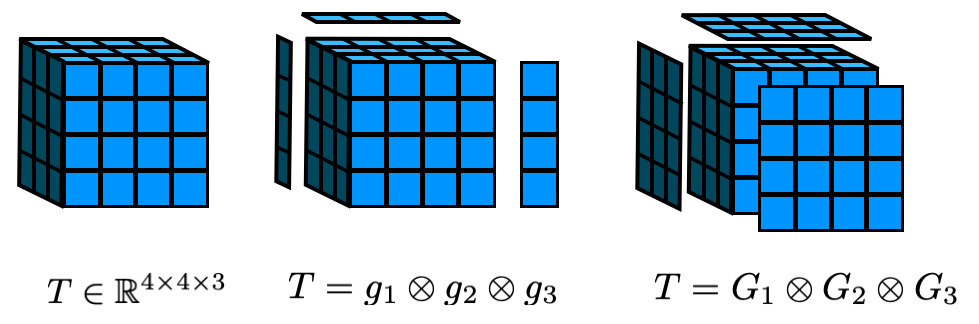
\includegraphics[width=\textwidth]{2_bknd/tensor_decomps.png}
	\caption[Tensor decompositions]{\label{fig:cp_decomp} CP-style and Tucker decompositions of an arbitrary tensor.}
\end{figure}
\todo{fig: this figure is just wrong, need to update}

A more recent decomposition, the \textit{Tensor Train} decomposition (TT) \citep{oseledets2011tensor}, defines an element of the tensor as
\begin{align}
\cX(x_1,\ldots,x_d) = A_1(x_1)\cdots A_d(x_d)
\end{align}
where $x_i \in \left\{1,\ldots, n_i\right\}$, and $A_i(x_i) \in \RR^{r_{i-1} \times r_{i}}$ for each $i \in \{1,\ldots,d\}$ are called the \textit{cores} of the tensor train, with $r_0 = r_d = 1$. Equivalently, the full tensor is written as:
\begin{align}\label{eq:fullTT}
	\cX &= \sum_{k_0 = 1}^{r_0} \cdots \sum_{k_d = 1}^{r_d} A_1(k_0,:,k_1) \otimes \cdots \otimes A_d(k_{d-1},:,k_d) 
\end{align}
where $A_i \in \RR^{r_{i-1}\times n_i \times r_i} $. 
This format requires $O(dnr^2)$ storage, but has two major advantages over the CP format. First, finding the TT-rank (the smallest set of $r_i$'s that satisfy the decomposition with equality) of any arbitrary tensor is tractable, and as such all tensors can be efficiently rewritten in the TT format. Second, projecting arbitrary tensors onto the TT format of a fixed rank requires only a set of QR and singular value decompositions \citep{oseledets2011tensor}. This projection, \textit{TT-rounding}, additionally allows for a given TT tensor of some rank to be projected onto the space of TTs with lower rank, and requires $O(dr^3)$ computational complexity. Separately, specific tensor train constructions have recently been identified as forms of general recurrent networks \citep{khrulkov2018generalized}.
\begin{figure}
	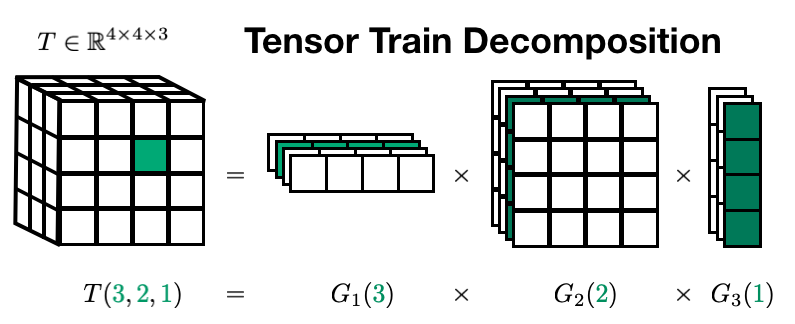
\includegraphics[width=\textwidth]{2_bknd/tt_decomp.png}
	\caption[Tensor train decomposition]{\label{fig:ttdecomp} Visualization of a tensor train decomposition.}
\end{figure}
\todo{figure quality, export from keynote and use trim/clip}
We denote a tensor operator $\tG$ as a grouping of tensor modes into an ``input" and ``output" list, such that $\tG \in \RR^{(n_1^{in},\times\ldots\times,n_d^{in}) \times (n_1^{out},\times\ldots\times,n_d^{out})}$. This operator $\tG$ can be seen as the TT representation of a matrix $W \in \RR^{(n_1^i\cdots n_d^i) \times (n_1^o\cdots n_d^o)}$. In \cite{novikov2015tensorizing}, authors use this formulation to directly compress the weight layers in neural networks. Cores in the operator are indexed by both an input and output index, i.e., $A_i(x_i,y_i) \in \RR^{r_{i-1}\times r_i}$, where $x_i \in [1,\ldots,n_i^{in}], y_i \in [1,\ldots,n_i^{out}]$.

Common operations upon tensor trains require \textit{matricizing} the cores of the TT format. Here, we define the left matricization of core $A_i(x_i)$ as $A_i^L \in \RR^{r_{i-1}n_i \times r_i} $ and the right matricization similarly.
Other desirable operations are fully supported by the format as well,
including most linear algebra operations such as summations,
multiplications, Frobenius norms,
and decomposition into the format via an iterative higher-order SVD procedure.
For brevity in this thesis, we refer interested readers
to the original tensor train proposal and citations above.

\subsection{Differential Geometry of Tensor Trains}
Tensor trains with fixed TT-ranks form a Riemannian submanifold of $\RR^{n_1 \times \cdots \times n_d}$ \cite{lubich2015time, holtz2012manifolds}:
\begin{align}\label{eq:riem}
	\cM_r := \{ \cX \in \RR^{n_1 \times \cdots \times n_d} \text{ with TT-ranks\ } r_0,\ldots,r_d\} 
\end{align}
Optimizing a function with respect to a Riemannian manifold-valued variable amounts to computing a free derivative in the ambient space, projecting the gradient to the tangent space of the current iterate, and using the (retraction) exponential map to compute the next iterate.
The authors in \cite{novikov2016exponential} use this procedure to more effectively learn a model of all exponentially many interactions in a linear model.


\section{Probability and Independence}

A random variable $X$ is a mapping from each element in an outcome space $x \in X$ to a real number $\RR$. This mapping is generally written as $p(x):=\PP(X=x), x \in X$ to denote the distribution over possible realizations $x$ of $X$. $X$ may also denote a \textit{set} of random variables $X:=\{x_i\}_{i=1}^n$, where a draw from the distribution over $X$ results in a vector $x$ of dimension $n$.
The \textit{expectation} of a random variable $\EE[X]$ is the ``weighted average'' over all outcomes. For discrete variables (which will be our main focus with expectations), 
\begin{align}
\EE[X] = \sum_{x\in X} x\cdot p(x)
\end{align}
The properties of distributions below extend to measures of expectations among multiple variables, with some caveats mentioned in specific chapters as needed.

Over a set of random variables $X$ and $Y$, the distribution $p(x,y):= \PP(X=x,Y=y)$ is the \textit{joint} distribution both variables $(X,Y)$. The \textit{marginal} distribution for $x$ is computed by ``summing out'' $y$, i.e.,
\begin{align}
p(x) = \PP(X=x) &= \sum_y \PP(X=x,Y=y) = \sum_y p(x,y) \\
&= \int p(x,y) dy
\end{align}
We say that the random variables $X$ and $Y$ are \textit{independent} if their joint distribution is equal to the product of their marginals: $p(x,y) = p(x)p(y)$.
Intuitively, a draw from one distribution has no impact on the draw from the other. In the case where the variables are \textit{dependent}, the distributions are linked. The dependent draw is defined by the \textit{conditional} distribution $p(y|x)$. Then, a joint distribution can factor as an iterative draw first from $p(x)$ followed by from $p(y|x)$: $p(x,y) = p(x)p(y|x)$. Importantly, this dependence is commutative: it is also true that $p(x,y) = p(y)p(x|y)$. When $p(y|x) = p(y)$, we say that $Y$ is independent of $X$. This commutativity leads to the formulation of Bayes' Rule:
\begin{align}
    p(y|x) = \frac{p(x|y)p(y)}{p(x)}
\end{align}
This form is used throughout statistics and machine learning. In most settings, we are interested in estimating some parameters $\theta$, or distribution over parameters $p(\theta)$, given a distribution over data $p(x)$. Applying Bayes' Rule:
\begin{align}
    p(\theta|x) = \frac{p(x|\theta)p(\theta)}{p(x)}
\end{align}
Where $p(x|\theta)$ is the \textit{likelihood} of observing the data $x$ given some parameter set, $p(\theta)$ is the \textit{prior} assumption on the base distribution over parameters, $p(x)$ is the marginal over all data (treated as a normalizing constant), and $p(\theta|x)$ is the \textit{posterior} distribution over the parameters given some data.
Alternatively, we wish to update our estimation of the parameters $\theta$ from $p(\theta)$ to $p(\theta|x)$ given some observations $x$ that change our beliefs about the parameter space.
Maximum a posteriori (MAP) estimation attempts to find the parameters that maximize this posterior, using Bayes' rule for tractable computation and estimation.
\begin{align}\label{eq:map}
	\max_\theta p(\theta|x) = \max_\theta \frac{p(x|\theta)p(\theta)}{p(x)} =  \max_\theta p(x|\theta)p(\theta)
\end{align}
If we have some samples $\{x_i\}_{i=1}^n$ from the data distribution that comprise a dataset,
then we have the following equivalent log-transformed model:
\begin{align}
	\max_\theta \sum_{i=1}^n \log p(x_i|\theta) + \log
\end{align}

\subsection{Conditional Independence} 
With three or more variables, independence relations among variables may be determined by which variables are being conditioned upon. 
\begin{definition}[Conditional Independence]\label{def:condindep}
For three random variables $X,Y,Z$, we say that 
$Y$ is \textit{conditionally independent} of $X$ given $Z$, written as $Y \indep X | Z$, if
\begin{align}
    p(y,x|z) = p(y|z)p(x|z).
\end{align}    
\end{definition}
Intuitively, once you know $Z$, $X$ provides no additional information in predicting $X$. This can also be written as $p(y|x,z)=p(y|z)$.



\paragraph{Graphs.}
With a larger number of variables, independence relations can be difficult to define with this notation. \textit{Graphs} are commonly used in place.
Graphs $G \in \cG$ are defined by their vertex and edge sets $G:=(E,V)$.
The vertices $V$ correspond to some random variables $X,Y,Z,\ldots$, or $X_1,\ldots,X_n$. 
An \textit{undirected} graph is one in which the existence of an edge $e_{ij}$ implies the existence of edge $e_{ji}$.
Within a \textit{probabilistic graphical model}, an edge $e_{ij}$ implies a \textit{conditional dependence}. The omission of a particular edge thus has an explicit meaning:
\begin{align}
    e_{ij} \not\in E \iff X_i \indep X_j | X_{V\setminus(i,j)}
\end{align}
Where $V\setminus(i,j)$ is the rest of the variables in the set and graph. A graph with these independence relations is also referred to as a Markov graph: pairwise conditional independence relations imply \textit{global} conditional independence relations: for any sets of variables $A,B,C$, if $C$ ``separates'' $A$ and $B$, 
While directed graphs are used and are of independent interest, in this thesis we focus on undirected graphs.

\paragraph{Multivariate Gaussians.}
Extending the typical univariate Gaussian distribution $p(x) = \frac{1}{\sqrt{2\pi\sigma^2}}e^{-(x-\mu)^2/2\sigma^2}$ defined by mean and variance parameters $\mu,\sigma^2$, we have the following density function for multivariate Gaussian distributions over $n$ variables, with realizations as the vector $\mathbf{x}:=[x_1,\ldots,x_n]^\top$:
\begin{align}\label{eq:mvgauss}
    p(x_1,\ldots,x_n) = \frac{1}{\sqrt{(2\pi)^n|\Sigma|}} \EXP\left(\frac{1}{2}(\mathbf{x} - \mathbf{\mu})^\top \Sigma^{-1} (\mathbf{x} - \mathbf{\mu})\right)
\end{align}
Where $\mathbf{\mu}$ is the vector of means for each individual variable, and $\Sigma$ is the $n\times n$ \textit{covariance} matrix describing the second-order interactions among the variables. 
The tractability of both computing the density and estimating it in typical likelihood estimation frameworks makes the multivariate Gaussian a particular attractive prior used in many applications,
including estimating independence.
Specifically, 
\begin{theorem}\label{thm:mvnindep}
    Let $X$ be governed by a multivariate Gaussian as defined in \ref{eq:mvgauss}. Then it holds that
    \begin{align}
        \Sigma_{ij} = 0 \iff X_i \indep X_j
    \end{align}
\end{theorem}
Complete independence among variables is often not possible and in most settings not valuable. However, a more powerful result for conditional independence exists.
\begin{theorem}\label{thm:mvncondindep}
    Let $X$ be governed by a multivariate Gaussian as defined in \ref{eq:mvgauss}, and $\Omega:=\Sigma^{-1}$ be the precision matrix. Then it holds that
    \begin{align}
        \Omega_{ij} = 0 \iff X_i \indep X_j | X_{\setminus(i,j)}
    \end{align}
\end{theorem}
This immediately yields that the precision matrix encodes the edges of the probabilistic graphical model over the variables. Estimating these dependencies is thus equivalent to estimation of the precision matrix.

\subsection{Estimating Parameters and Measures Over and Among Distributions}
When samples are drawn from a particular family of distributions, a number of methods exist to estimate the parameters that fit that data best. 
MAP estimation and maximum likelihood estimation as described above are typically used,
but in many cases their standard forms do not yield
parameters that reveal independence, i.e., it is often impossible for standard
methods to result in a parameter estimate of zero.

To determine the relationship among two random variables, measures such as the Pearson correlation coefficient, and Spearman and Kendall rank coefficients \citep{myers2013research} are frequently used, with values close to zero suggesting a low importance, and a value close to 1 suggesting perfect dependence. However,
these measures are only applicable with specific assumptions about the possible dependencies between the variables: Pearson coefficients can only identify linear dependencies, and rank coefficients typically fail with non-monotonic dependencies (e.g., periodic functions). These methods can be computed pairwise among all variables among a set of variables with size greater than 2, however, to estimate conditional dependencies typically requires the estimation of \textit{partial} coefficient measures.
Additionally, while results similar to Theorem~\ref{thm:mvncondindep} exist under specific assumptions ,
practical estimation does not often yield exact zeros,
and estimating all partial coefficients separately can be computationally heavy.

With some assumptions, \textit{sparse} recoveries are possible while estimating ALL conditional independencies. Following the results from multivariate Gaussians above,
a \textit{penalized} version of a maximum likelihood estimate can be recovered through the following \textit{graphical lasso} \cite{friedman2008sparse} formulation:
\begin{align}\label{eq:glasso}
    \hat{\Omega} = \min_{\Omega \succeq} \tr(S\Omega) + \log|\Omega| + \lambda||\Omega||_1
\end{align}
With $S$ being the sample covariance of the data samples, and $\lambda$ a penalization weight. This $\ell_1$ penalization has been shown to be easy to compute, and a number of alternative versions have been proposed with varying theoretical properties and recovery guarantees~\citep{cai2011constrained,yuan2010high}.
Particularly interesting are extensions to \textit{nonparanormal} distributions, which allow for a much larger set of graphs to be estimated over other distributions via a rank covariance matrix, generalizing the pairwise rank and distance coefficients above \cite{liu2009nonparanormal,xue2012regularized}.

The distributional assumptions needed for all of these methods, however, are often completely unknown in practice, or the data represent highly complex densities and functions that cannot be represented by simple exponential families or rank-based measures.
Newer measures of \textit{nonparametric} estimations of dependence have been developed, such as distance correlation and kernel-based coefficients \cite{abc}, but they tend to either only test for independence and not strength of functional relationship, or have complex instantations or asymptotic theories, making them difficult to deploy and rely upon in practice.

A recent coefficient, the Chatterjee coefficient, has been demonstrated to have a number of desirable properties, and has been further developed into an elegant method for testing conditional independence~\citep{abc,abc}. 
Particularly,
no conditional densities need to be estimated,
it can be computed in $O(n\log n)$ time where $n$ is the number of data samples,
it asymptotically to 0 for conditional independence, and 1 for measurable functions,
and it requires \textit{absolutely no assumptions} on the law over the random variables.
For arbitrary variables random $X,Y,Z$, where $Y$ is univariate and $X,Z$ can be multivariate of any size, the conditional coefficient is given  by
\begin{align}\label{eq:contcodec}
    T(Y,X|Z) = \frac{\int\EE\left[\VAR(\PP(Y\geq t)|X,Z)|Z)\right]d\mu(t)}{\int\EE\left[\VAR(\II\{Y\geq t\}|Z\right] d\mu(t)}
\end{align}
In the following chapters we will take advantage of these properties. Critically, without a specific procedure, identifying the conditioning set for a particular independence test is exponential. If we wish to find which variables $X_1,\ldots,X_n$ are sufficient for creating independence between some outcome $Y$ and the rest of the variables, na\"ively we would need to test all possible subsets.
An advantage of the coefficient of dependence in \cite{abc} is that it admits a linear time algorithm for iteratively building the sufficient set, naturally enabling an algorithm for constructing a Markov graph over the variables of interest.

\subsection{Hypothesis Testing}

Statistical hypothesis testing involves formally defining and testing a hypothesis about the world.
A prior ``null'' assumption is defined. The \textit{null} hypothesis, $H_0$
represents the default assumption or expectation
that there is no relationship or distinction among
the true population states,
whereas the \textit{alternative} hypothesis, $H_A$,
describes the world in which some hypothesized 
relationship or distinction does exist.
Testing proceeds by collecting observations
of the variables of interest,
computing a \textit{test statistic},
and comparing that statistic against
a prior \textit{null distribution}.
If the test statistic is larger
than a predefined critical value,
the null hypothesis is rejected:
there is reasonable evidence to suggest
the alternative may be true.
When we fail to reject the null,
there is insufficient evidence to support
the alternative claim.

The form of the test statistic and null distribution
are defined by the specific hypothesis being tested,
as well as the prior assumptions about the parameters
of interest and data collected.

\paragraph{Example: Testing a difference of means.} 
Say we have collected samples from two different groups,
representing the height of each person in the group.
Our task is to determine if the average height
of the two groups is significantly different from each other.
Na\"ively, we can compute the averages of the two groups and compare.
In practice these averages will never be equal, so how can we 
more rigorously determine if we should consider some measured difference
significant enough to say the groups are different?
We can set up the following hypothesis test.

Let $\mu_1$ be the true \textit{population mean} of group 1,
and $\mu_2$ the true population mean of group 2.
Our hypotheses are:
\begin{align}
H_0: \mu_1 = \mu_2 \qquad H_A: \mu_1 \neq \mu_2
\end{align}
Let us assume we have collected the same number of samples from each group,
$n$, and that the means of the collected samples are $\hat{\mu}_1$ and $\hat{\mu}_2$,
and the standard deviations are $s_1$ and $s_2$.
Then the test statistic
\begin{align}
t = \frac{\hat{\mu}_1 - \hat{\mu}_2}{\sqrt{\frac{s_1^2 + s_2^2}{n}}}
\end{align}
follows a $t$-distribution with $n-1$ degrees of freedom,
\textit{if} there is no difference between the means.
Comparing the value of the measured statistic over the observed data
to the corresponding $t$-distribution allows
us to determine how likely or unlikely it is that 
our observation follows the law that the means are equal.
If we want our test to accurately identify
a difference between means 95\% of the time,
we can set our threshold $t^*$ (critical value) for rejecting the null
to be the point where $\PP(t \geq t^*) \geq 0.95$.

Importantly, the value of the $t$-statistic and corresponding
distribution and critical value are extremely
dependent on the number of samples $n$ acquired for the test.
As we will see, in cases where the number of samples is 
very small and our hypothesis describes 
a subtle difference between groups,
novel tests and procedures are necessary
to effectively identify those differences.





\begin{verbatim}
basics
    form
    measures
    continuous, traditionally want "gap" to be at least "alpha" large
    example: means

some of the measures described above have specific 
guarantees when evaluated under
standard hypothesis testing frameworks...

a common test: likelihood ratio...

subsec: scan statistics
\end{verbatim}


\section{Deep Networks, Optimization, and Objectives}
The form of the function $f_\theta$ in~\eqref{eq:learning}
is critical in determining both
the types of optimization methods
that may identify a solution,
and the particular minimizer identified.
In the learning methods that follow,
$f$ will typically take the form of 
a deep neural network.
The advantages
and successes of deep neural networks
rely heavily on their ease of optimization:
the \textit{computation graph} that 
underlies the neural network
allows for gradients
to be computed by parts
and accumulated via the chain rule.

Consider a simple function $f_\theta(x)$
that is defined as a linear combination of 
some parameters $\theta:=w, w\in \RR^d$ with $x\in \RR^d$ followed by 
a differentiable, nonlinear scalar \textit{activation} function $a(\cdot)$:
\begin{align}
	f_\theta(x) := a(w\cdot x)
\end{align}
If we have some estimate of the parameters $\theta:=w$,
then the gradient of the full network with respect to those parameters is
\begin{align}
	\frac{df}{d\theta} = \frac{df}{da}\frac{da}{dw}
\end{align}
where $df/da$ is the (known) derivative of the \textit{activation} function,
and $da/dw$ is exactly $x$, the derivative of a linear function.
With a direction of descent,
we can update the parameters via some update to minimize the functional $f$ of interest:
\begin{align}
	\theta_{t+1} = \theta_t + g(\theta_t,x)
\end{align}
where $g(\cdot)$ is some function of the full derivative $g(\cdot) := g(\nabla f_\theta(x))$,
and $\theta_t$ are the current parameter estimates.
Optimization proceeds and terminates when a certain amount
of iterations $t$ have completed,
or some stopping criterion has been reached,
typically that the gradient is small,
indicating that a minima has been identified.

\begin{verbatim}
full gradients not feasible, large samples,
hessians
\end{verbatim}



This formulation and gradient update generalize
to extremely large and complex stacks
of operations, and are what have enabled
the enormous success and ubiquity of learning
methods to this day.
Importantly,
the final minima identified can 
vary significantly based on the particular form 
of the function $f_\theta$, and,
in the case where the function $f$ is
not \textit{convex},
it can also depend on
the initial estimate $\theta_0$ at initialization.


forms of $f$, architectures
	architecture search
	initializations
		lottery ticket
		


\begin{verbatim}
networks
    objective
how to minimize?
    general optimization?
    gradients
    stochastic grad
\end{verbatim}

\subsection{Losses and Probability Measures}
loss functions, objectives
arbitrary distances
MSE
regularizers

probabilistic distances
KL
mutual information
MMD

\subsubsection{Optimal Transport}	
\begin{verbatim}
	OT definition
	earth movers bknd
	continuous
	discrete
	2d bknd
	when metric is abc,...
	nice props, existing work, more in chapter 6
    OT can be framed as a linear program....
\end{verbatim}
    

